\section{Introduzione}

L'iterazione 1 ha come scopo quello di identificare le componenti dal modello dei casi d'uso, 
applicando le euristiche di early design: verrà perfezionata la specifica dei componenti 
progettati durante l'iterazione 0 al fine di da definire meglio l'architettura software. 
È stato costruito lo scheletro dell'applicazione tramite la specifica delle differenti classi 
popolate nelle seguenti iterazioni.

Inizialmente, durante lo sviluppo dell'iterazione 0, il sistema nella sua totalità è stato 
visualizzato come una unica componente e sono stati 
introdotti gli attori, ognuno dei quali definito come un'entità esterna. In seguito sono stati 
sviluppati tutti i casi d'uso che riassumono il funzionamento del sistema, i quali verranno, 
nell'Iterazione 1, raccolti e raggruppati secondo un preciso criterio e affinità. 

Vengono inoltre introdotti componenti e sottocomponenti di controllo di ciascun gruppo, o 
alternativamente componenti di dati; per ognuna di esse nascono parallelamente le classi 
candidate e le relazioni che le legano. 

Per ogni caso d'uso che ha una interazione diretta con un attore esterno viene introdotta 
un'interfaccia per le operazioni visibili esternamente, ovvero le API, offerte o richieste 
dal componente o sottocomponente corrispondente, in base alla direzione dell'interazione. 

Ogni variabile input da un attore, specificata nella descrizione di un caso d'uso, 
definisce un parametro di input dell'operazione dell'interfaccia corrispondente. 
Ogni variabile output per un attore specificata nella descrizione di un caso d'uso 
definisce un parametro di ritorno dell'operazione dell'interfaccia corrispondente 
(se modalità sincrona) o un input di un'operazione dell'interfaccia di callback (se modalità asincrona) dell'attore. 

Viene scomposto il sistema in sottosistemi e componenti, applicando pattern e 
stili architetturali, per poi distribuire le componenti su nodi computazionali basati su 
uno sviluppo fisico del sistema.



\newpage

\section{Casi d'uso}
I casi d'uso vengono raggruppati in tre macro categorie in base a un criterio di affinità:
i primi sono relativi all'autenticazione dell'utente, i secondi sono relativi a tutto
ciò che riguarda l'ambito musicale, ed infine quelli relativi all'account personale e lato social. 
Di seguito un elenco dettagliato dei casi d'uso suddivisi come anticipato.

\subsection{Autenticazione}
    \begin{itemize}
        \item \textbf{UC1:} Sign up 
        \item \textbf{UC2:} Sign in
        \item \textbf{UC3:} Sign out 
    \end{itemize}


\subsection{Musica}
\begin{itemize}
    \item \textbf{Brano:} in questa sezione rientrano tutti i casi d'uso relativi ai brani.
    \begin{itemize}
        \item \textbf{UC4:} Cerca brano
        \item \textbf{UC5:} Cerca album
        \item \textbf{UC6:} Cerca Artista
        \item \textbf{UC7:} Scarica brano
        \item \textbf{UC8:} Like al brano
        \item \textbf{UC19:} ``Discover'' e classifiche
    \end{itemize} 
    
    \item \textbf{Playlist:} in questa sezione rientrano tutti i casi d'uso relativi alla creazione e gestione delle playlist.
    \begin{itemize}
        \item \textbf{UC9:} Aggiungi brano a playlist
        \item \textbf{UC15:} Visualizza playlist 
        \item \textbf{UC16:} Crea nuova playlist 
        \item \textbf{UC17:} Elimina playlist
        \item \textbf{UC18:} Modifica playlist
    \end{itemize}
    
    \item \textbf{Artista:} in questa sezione rientrano tutti i casi d'uso relativi alla gestione del profilo artista.
    \begin{itemize}
        \item  \textbf{UC20:} Crea pagina artista 
        \item  \textbf{UC21:} Visualizza pagina artista 
        \item  \textbf{UC22:} Aggiungi brano 
        \item  \textbf{UC23:} Aggiungi album 
        \item  \textbf{UC24:} Personalizza pagina artista 
        \item  \textbf{UC25:} Consulta anagrafica
    \end{itemize} 
\end{itemize}

\subsection{Account}
\begin{itemize}
    \item \textbf{Personale:} in questa sezione rientrano tutti i casi d'uso relativi alla gestione delle informazioni nel proprio profilo personale.
    \begin{itemize}
        \item \textbf{UC12:} Visualizza informazioni profilo 
        \item \textbf{UC13:} Modifica profilo 
        \item \textbf{UC14:} Elimina profilo 
    \end{itemize}
    
    \item \textbf{Amici:} in questa sezione rientrano tutti i casi d'uso relativi alla parte social.
    \begin{itemize}
        \item \textbf{UC10:} Cerca Utente 
        \item \textbf{UC11:} Aggiungi Utente 
    \end{itemize}
\end{itemize}

\newpage
\section{System Diagram}
In figura sono rappresentate tutte le interfacce richieste ed esposte dal nostro sistema. Inoltre,
i casi d'uso sono stati raggruppati indicando il nome dell'interfaccia che permetterà di implementare
il particolare caso d'uso.


\newpage

\section{UML Component Diagram}
Il Component Diagram in UML ha come obiettivo quello di mostrare la struttura
del sistema software, descrivendo i singoli componenti, le relative interfacce 
e le dipendenze. 
La rappresentazione del sistema è stata gestita partendo da una
una componente centrale, il server del sistema, alla quale si collegano il database e la parte front-end.


\begin{figure}[H]
    \centering
    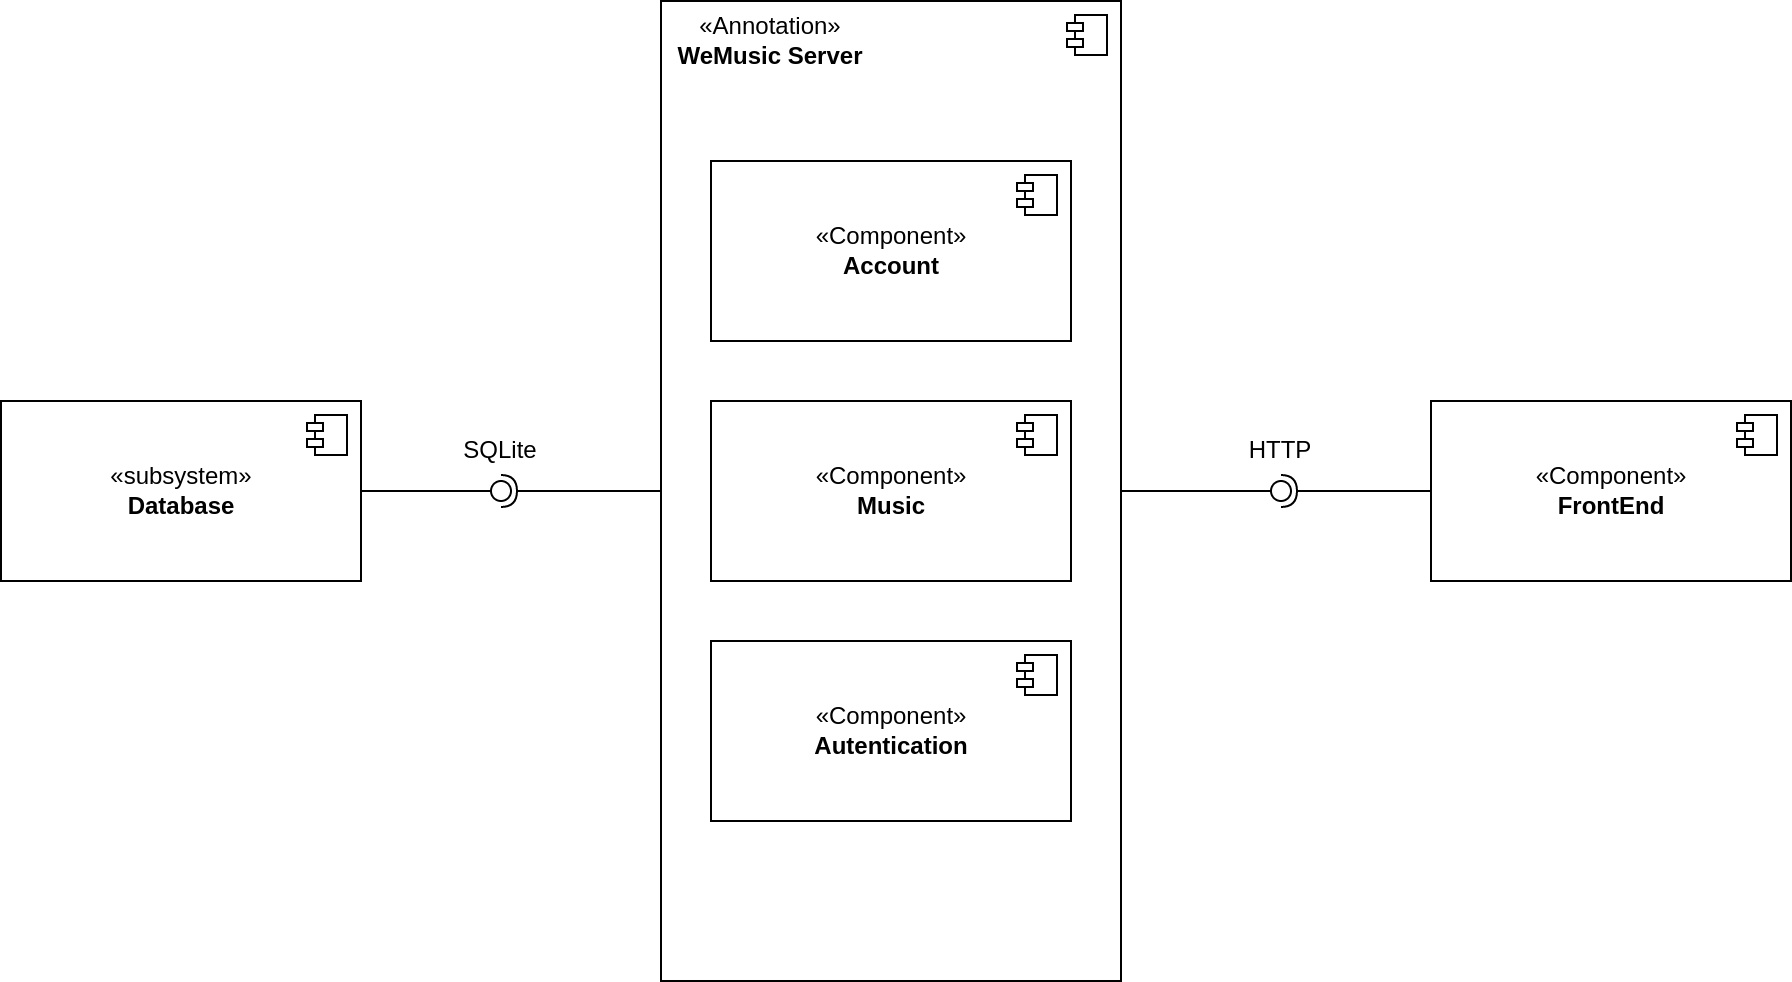
\includegraphics[scale=0.20]{component_diagram_v00.png}
    \caption{UML Component Diagram}
    \label{fig-uml-component-diag}
\end{figure}



\newpage

\section{UML Class Diagram}
Il Class Diagram in UML permette di descrivere il sistema 
visualizzando i diversi tipi di oggetti all'interno di esso e le relazioni 
statiche che esistono fra loro: sono descritte in maniera più approfondita 
le tre componenti già precedentemente analizzate, ovvero Account, Musica e 
Autenticazione.
In questo caso vengono rappresentati in unico diagramma il Data Class Diagram 
e l'Interface/Package Diagram.
Il primo descrive le classi che compongono la struttura dell'applicazione,  
le entità presenti al suo interno; il secondo rappresenta i package che 
riassumono la struttura logica dell’applicazione con i metodi implementati. 

\begin{figure}[H]
    \centering
    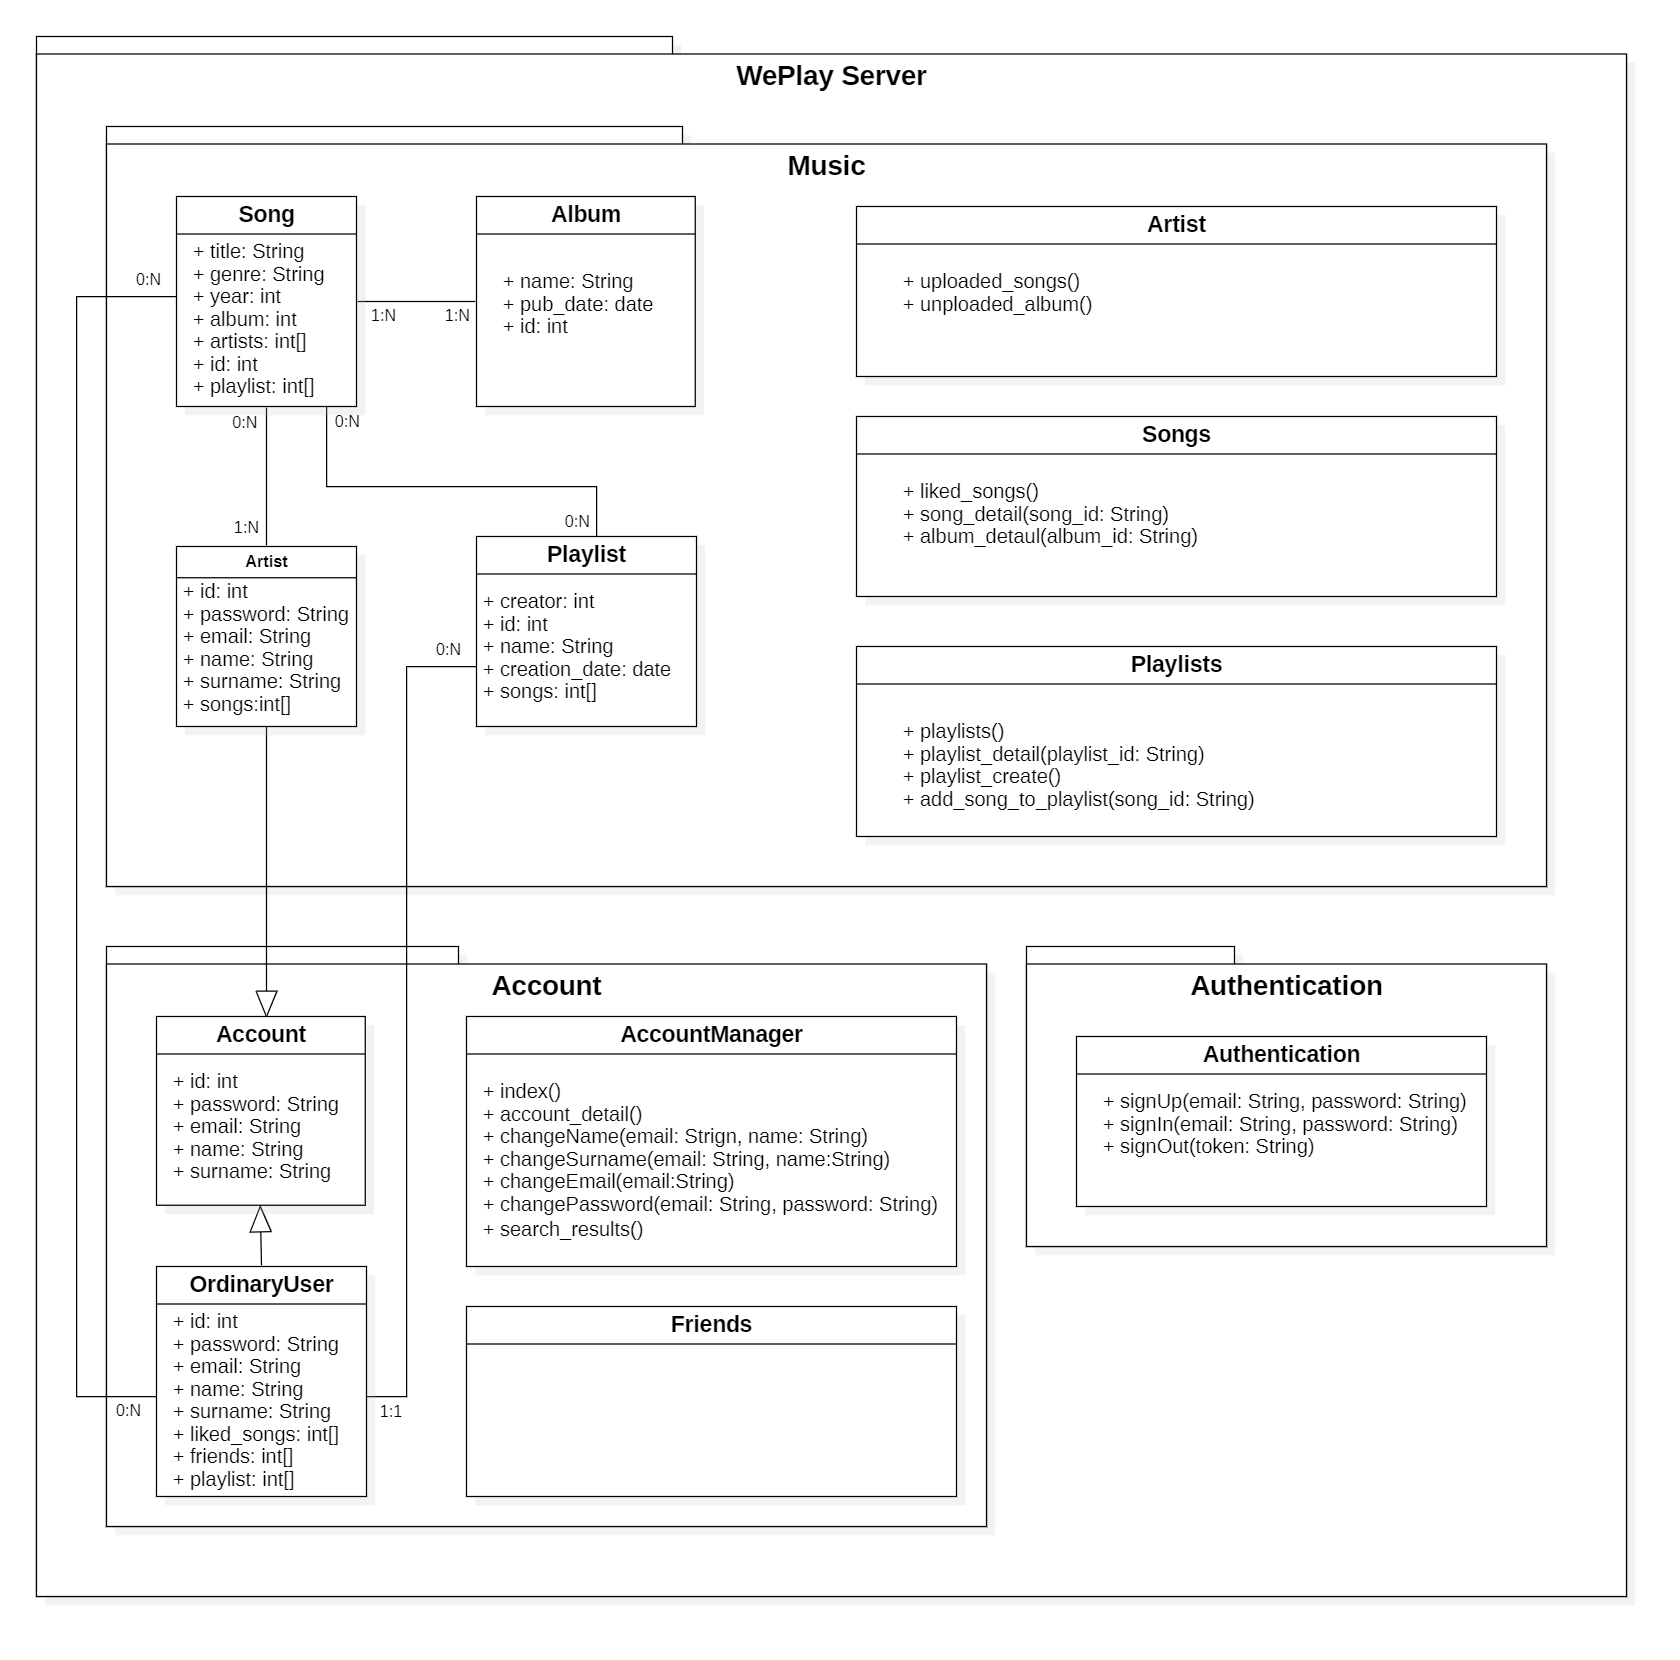
\includegraphics[scale=0.37]{images/ClassDiagram_ver1.png}
    \caption{UML  Class Diagram}
    \label{fig-uml-class-diag}
\end{figure}
\newpage
